\documentclass{article}
\usepackage[utf8]{inputenc}
%\usepackage[spanish,es-tabla,es-nodecimaldot]{babel}
\usepackage{enumitem}
\usepackage{tikz}
\usetikzlibrary{automata, positioning, arrows}
\tikzset{ ->, % makes the edges directed
>=stealth', % makes the arrow heads bold
node distance=2cm, % specifies the minimum distance between two nodes. Change if
necessary.
every state/.style={thick, fill=gray!10},
% sets the properties for each ’state’ node
initial text=$ $ }

\title{Exercises from Introduction to the Theory of Computation. Michael Sipser.}
\author{Ana Maritza Bello Yañez}
\date{\today}

\begin{document}
\maketitle

\textbf{1.1} The following are the state diagrams of two DFAs, $M_1$ and $M_2$ . Answer
the following questions about each of these machines.


\begin{figure}[h!]
\centering
    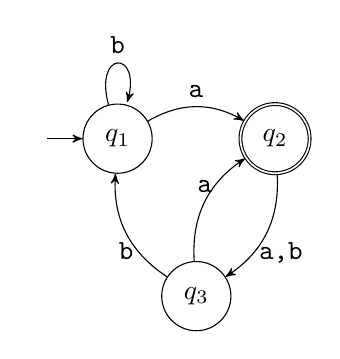
\begin{tikzpicture}
        \node [state, initial] (q1){$q_1$}; 
        \node [state, accepting,right of = q1] (q2){$q_2$};
        \node [state, below of = q1, xshift=1cm] (q3){$q_3$};
            
        \draw (q1) edge[loop above] node{\texttt{b}} (q1);
        \draw (q1) edge[bend left, above] node{\texttt{a}} (q2);
        \draw (q3) edge[bend left, below] node{\texttt{b}} (q1);
        \draw (q2) edge[bend left, below] node{\texttt{\ \ a,b}}(q3);
        \draw (q3) edge[bend left, above] node{\texttt{a}} (q2);
    \end{tikzpicture}
\caption{$M_1$}
\end{figure}
    

\begin{itemize}

\item What is the start state? \\
\textbf{R: } $q_0 = q_1 \in Q$

\item What is the set of accept states? \\
\textbf{R: } $F = \{q_2\}$

\item What sequence of states does the machine go through on input \texttt{aabb}
? \\
\textbf{R: }
\begin{enumerate}
    \item Start state in $q_1$
    \item Read \texttt{a}, follow transition from $q_1$ to $q_2$
    \item Read \texttt{a}, follow transition from $q_2$ to $q_3$
    \item Read \texttt{b}, follow transition from $q_3$ to $q_1$
    \item Read \texttt{b}, follow transition from $q_1$ to $q_1$
\end{enumerate}

\item Does the machine accept the string \texttt{aabb}? \\
\textbf{R: } No, it doesn't. It rejects it because at the end of the input,
$M_1$ is in state $q_1$ which is not an accept state.

\item Does the machine accept the string $\varepsilon$? \\
\textbf{R: } If it does. Because when an empty string is accepted, the initial
state, which is also the accept state, remains the same.
\end{itemize}

\begin{figure}[h!]
\centering
    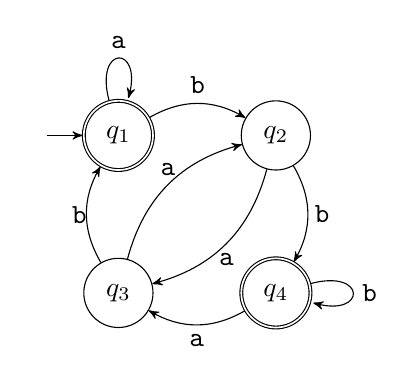
\begin{tikzpicture}
        \node [state, initial, accepting] (q1){$q_1$}; 
        \node [state, right of = q1] (q2){$q_2$};
        \node [state, below of = q1] (q3){$q_3$};
        \node [state, accepting, right of = q3] (q4){$q_4$};
            
        \draw (q1) edge[loop above] node{\texttt{a}} (q1);
        \draw (q4) edge[loop right] node{\texttt{b}} (q4);
        \draw (q1) edge[bend left, above] node{\texttt{b}} (q2);
        \draw (q2) edge[bend left] node{\texttt{\ \ b}} (q4);
        \draw (q2) edge[bend left, below] node{\texttt{a}}(q3);
        \draw (q3) edge[bend left, above] node{\texttt{a}} (q2);
        \draw (q3) edge[bend left] node{\texttt{b\ \ }} (q1);
        \draw (q4) edge[bend left, below] node{\texttt{a}} (q3);
    \end{tikzpicture}
\caption{$M_2$}
\end{figure}

\begin{itemize}

\item What is the start state? \\
\textbf{R: } $q_0 = q_1 \in Q$

\item What is the set of accept states? \\
\textbf{R: } $F = \{q_1, q_4\}$

\item What sequence of states does the machine go through on input
\texttt{aabb}? \\
\textbf{R: }
\begin{enumerate}
    \item Start state in $q_1$
    \item Read \texttt{a}, follow transition from $q_1$ to $q_1$
    \item Read \texttt{a}, follow transition from $q_1$ to $q_1$
    \item Read \texttt{b}, follow transition from $q_1$ to $q_2$
    \item Read \texttt{b}, follow transition from $q_2$ to $q_4$
\end{enumerate}

\item Does the machine accept the string \texttt{aabb}? \\
\textbf{R: } Yes, it does, because the state at the end of the string is $q_4$
which is an accept state.

\item Does the machine accept the string $\varepsilon$? \\
\textbf{R: } Yes, because the start state is also an accept state.

\end{itemize}

\pagebreak
\textbf{1.2} Give the formal description of the machines M1 and M2 pictured in
Exercise 1. \\
\textbf{R: } 
\begin{center}
    $M_1 = ( Q, \sum, \delta, q_0, F)$, where 
\end{center}

\begin{enumerate}
    \item $Q = \{q_1, q_2, q_3\}$
    \item $\sum = \{\texttt{a,b}\}$
    \item $\delta$ is described as
    \begin{center}
        \begin{tabular}{c|cc}
            &   \texttt{a}     &   \texttt{b} \\
            \hline
            $q_1$   &   $q_2$   &   $q_1$   \\
            $q_2$   &   $q_3$   &   $q_3$   \\
            $q_3$   &   $q_2$   &   $q_1$
        \end{tabular}
    \end{center}
    \item $q_0 = q_1 \in Q$
    \item $F = \{q_2\}$
\end{enumerate}

\begin{center}
    $M_2 = ( Q, \sum, \delta, q_0, F)$, where 
\end{center}

\begin{enumerate}
    \item $Q = \{q_1, q_2, q_3, q_4\}$
    \item $\sum = \{\texttt{a,b}\}$
    \item $\delta$ is described as
    \begin{center}
        \begin{tabular}{c|cc}
            &   \texttt{a}     &   \texttt{b} \\
            \hline
            $q_1$   &   $q_1$   &   $q_2$   \\
            $q_2$   &   $q_3$   &   $q_4$   \\
            $q_3$   &   $q_2$   &   $q_1$   \\
            $q_4$   &   $q_3$   &   $q_4$
        \end{tabular}
    \end{center}
    \item $q_0 = q_1 \in Q$
    \item $F = \{q_1, q_4\}$
\end{enumerate}

\pagebreak
\textbf{1.3} The formal description of a DFA $M$ is
($\{q_1,q_2,q_3,q_4,q_5\}$,$\{\texttt{u},\texttt{d}\}$,$\delta$,$q_3$,$\{q_3\}$),
where $\delta$ is given by the following table. Give the state diagram of this
machine.

\begin{center}
\begin{tabular}{c|cc}
            &   \texttt{u}     &   \texttt{d} \\
    \hline
    $q_1$   &   $q_1$   &   $q_2$   \\
    $q_2$   &   $q_1$   &   $q_3$   \\
    $q_3$   &   $q_2$   &   $q_4$   \\
    $q_4$   &   $q_3$   &   $q_5$   \\
    $q_5$   &   $q_4$   &   $q_5$
\end{tabular}
\end{center}

\textbf{R: }
\begin{figure}[h!]
    \centering
        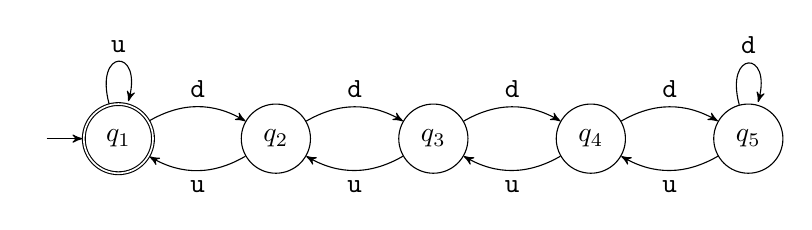
\begin{tikzpicture}
            \node [state, initial, accepting] (q1){$q_1$}; 
            \node [state, right of = q1] (q2){$q_2$};
            \node [state, right of = q2] (q3){$q_3$};
            \node [state, right of = q3] (q4){$q_4$};
            \node [state, right of = q4] (q5){$q_5$};
                
            \draw (q1) edge[loop above] node{\texttt{u}} (q1);
            \draw (q1) edge[bend left, above] node{\texttt{d}} (q2);

            \draw (q2) edge[bend left, below] node{\texttt{u}} (q1);
            \draw (q2) edge[bend left, above] node{\texttt{d}} (q3);

            \draw (q3) edge[bend left, below] node{\texttt{u}} (q2);
            \draw (q3) edge[bend left, above] node{\texttt{d}} (q4);

            \draw (q4) edge[bend left, below] node{\texttt{u}} (q3);
            \draw (q4) edge[bend left, above] node{\texttt{d}} (q5);

            \draw (q5) edge[bend left, below] node{\texttt{u}} (q4);
            \draw (q5) edge[loop above] node{\texttt{d}} (q5);
        \end{tikzpicture}
    \caption{State diagram of $M$}
    \end{figure}

\textbf{1.4} Each of the following languages is the intersection of two simpler
languages. In each part, construct DFAs for the simpler languages, then combine
them using the construction discussed in footnote 3 (page 46) to give the state
diagram of a DFA for the language given. In all parts $\sum = \{\texttt{a},
\texttt{b}\}$.

    \begin{enumerate}
        \item \{$w|w$ en has at least three \texttt{a}'s and at least two \texttt{b}'s\}
        \item \{$w|w$ has at exactly two \texttt{a}'s and at least two \texttt{b}'s\}
        \item \{$w|w$ has an even number of \texttt{a}'s and one or two \texttt{b}'s\}
        \item \{$w|w$ has an even number of \texttt{a}'s and each a is followed by at least one \texttt{b}\}
        \item \{$w|w$ has an even number of \texttt{a}'s and one or two \texttt{b}'s\}
        \item \{$w|w$ in has an odd number of \texttt{a}'s and ends with a \texttt{b}\}
        \item \{$w|w$ has even length and an odd number of \texttt{a}'s\}
    \end{enumerate}

\textbf{1.5} Each of the following languages is the complement of a simpler
language. In each part, construct a DFA for the simpler language, then use it to
give the state diagram of a DFA for the language given. In all parts $\sum =
\{\texttt{a}, \texttt{b}\}$.

\begin{enumerate}
\item \{$w|w$ does not contain the substring \texttt{ab}\}
\item \{$w|w$ does not contain the substring \texttt{baba}\}
\item \{$w|w$ contains neither the substrings \texttt{ab} nor \texttt{ba}\}
\item \{$w|w$ is any string not in $\texttt{a}^* \texttt{b}^*$\}
\item \{$w|w$ is any string not in \texttt{(ab$^+$)$^*$}\}
\item \{$w|w$ is any string not in \texttt{a$^*\cup$b$^*$}\}
\item \{$w|w$ is any string that doesn't contain exactly two \texttt{a}'s\}
\item \{$w|w$ is any string except \texttt{a} and \texttt{b}\}
\end{enumerate}

\textbf{1.6} Give state diagrams of DFAs recognizing the following languages. In
all parts the alphabet is \{\texttt{0,1}\}.

\begin{enumerate}
\item \{$w|w$ begins with a \texttt{1} and ends with a \texttt{0}\}
\item \{$w|w$ contains at least three \texttt{1}s\}
\item \{$w|w$ contains the substring \texttt{0101}, i.e., $w = x\texttt{0101}y$
for some $x$ and $y$\}
\item \{$w|w$ has length at least 3 and its third symbol is a \texttt{0}\}
\item \{$w|w$ starts with \texttt{0} and has odd length, or starts with
\texttt{1} and has even length\}
\item \{$w|w$ doesn't contain the substring \texttt{110}\}
\item \{$w|w$ the length of $w$ is at most 5\}
\item \{$w|w$ is any string except \texttt{11} and \texttt{111}\}
\item \{$w|w$ every odd position of $w$ is a \texttt{1}\}
\item \{$w|w$ contains at least two \texttt{0}s and at most one \texttt{1}\}
\item \{$\varepsilon$, $0$\}
\item \{$w|w$ contains an even number of \texttt{O}s, or contains exactly two
\texttt{1}s\}
\item The empty set
\item All strings except the empty string
\end{enumerate}

\end{document}
